\section{Implementation of NFC}
We have created a class called \lstinline|NfcForegroundActivity| which every activity that we want to enable \ac{nfc} on can extend. \lstinline|NfcForegroundActivity| enables the Foreground Dispatch System and contains methods which enables the activity to read and process \ac{nfc} tags.

\begin{figure}[H]
\centering
\includegraphics[width=0.55\linewidth, page=2]{img/nfcdiagram.pdf}
\caption{NFC class diagram}
\label{fig:nfcdiagram}
\end{figure}

\lstinline|NfcForegroundActivity| is an abstract class with one abstract method called \lstinline|onNfcScanned()|. All our activities inherits from this. This allows for a very easy way to handle the records that lie on the \ac{nfc} tag separately for each activity. Some of the important methods for \lstinline|NfcForegroundActivity| are shown in the diagram, and they are also explained in this section.

\subsection*{Foreground Dispatch System}
\label{sec:foreground}

When an activity uses Foreground Dispatch System, it forces priority over other activities when handling \ac{nfc} intents\citep{foregroundDispatch}. This enables us to handle intents when the user has the activity open and scans an \ac{nfc} tag.

\begin{lstlisting}[language=java, label=nfcForegroundOnCreate, caption={Initializing the pending intent}]
public NfcForegroundActivity(Context context) { 
    this.nfcAdapter = NfcAdapter.getDefaultAdapter(this.context);
    Intent intent = new Intent(this.context, ((Activity) this.context).getClass());
    this.nfcPendingIntent = PendingIntent.getActivity(this.context, 0, intent ,0);
}
\end{lstlisting}\todo{Tjek hvad der sker uden flag i applicationen}
\begin{description}
\item[Line 2] The default \ac{nfc} adapter is retrieved and saved.
\item[Line 4] A pending intent is created and saved for later use. This is necessary because the system must have an intent to populate when an \ac{nfc} tag is scanned.
\end{description}

\begin{lstlisting}[language=java, caption=Enable Foreground Dispatch System]
@Override
protected void onResume() {
	// foreground mode gives the current active application priority for reading scanned tags
	IntentFilter tagDetected = new IntentFilter(NfcAdapter.ACTION_TAG_DISCOVERED); 
	IntentFilter[] TagFilters = new IntentFilter[] { tagDetected };
	this.nfcAdapter.enableForegroundDispatch(this.context, this.nfcPendingIntent, TagFilters);
}

@Override
protected void onPause() {
    this.nfcAdapter.disableForegroundDispatch(this.context);
}
\end{lstlisting}
\begin{description}
\item[Line 2] \lstinline|onResume()| is run every time the activity is started.
\item[Line 4] An \lstinline|IntentFilter| is created. This particular filter tells the system that we want to override the behavior when an \ac{nfc} tag is scanned.
\item[Line 5] The filter is added to an array. This is required because you can have multiple filters.
\item[Line 6] Foreground Dispatch System is enabled with the pending intent created in \autoref{nfcForegroundOnCreate} and the intent filter.
\item[Lines 10-12] Every time the activity is paused we disable the Foreground Dispatch System.
\end{description}

\subsection*{Handling of NFC Intent}
When an \ac{nfc} tag is scanned the method shown in \autoref{lst:onNewIntent} is called. This method is a part of \lstinline|NfcForegroundActivity|.
\begin{lstlisting}[language=java, label=lst:onNewIntent, caption=\lstinline|onNewIntent()| method]
@Override
/* This method is called when an NFC tag is scanned */
public void onNewIntent(Intent intent) { 
    super.onNewIntent(intent);
    ArrayList<Record> records = this.nfcForeground.newIntentEvent(intent);
    if (records.size() > 0) {
        this.onNfcScanned(records);
    }
}  
\end{lstlisting}
\begin{description}
\item[Line 3] The intent parameter for \lstinline|onNewIntent()| is the pending intent that was created in \autoref{nfcForegroundOnCreate}.
\item[Line 5] The method \lstinline|newIntentEvent()| is run with the intent and a list of records is returned. \lstinline|newIntentEvent()| is shown below.
\item[Lines 6-7] If any records were found, \lstinline|onNfcScanned()| is called with these.
\end{description}

\begin{lstlisting}[language=java, label=lst:newIntentEvent, caption=\lstinline|newIntentEvent| parsing to records]
public ArrayList<Record> newIntentEvent(Intent intent) {
    Parcelable[] messages = intent.getParcelableArrayExtra(NfcAdapter.EXTRA_NDEF_MESSAGES);
    ArrayList<Record> foundRecords = new ArrayList<Record>();

    if (messages != null) {
        for (int i = 0; i < messages.length; i++) {

            List<Record> records = new Message((NdefMessage)messages[i]);

            for (int k = 0; k < records.size(); k++) {
                Record record = records.get(k);
                foundRecords.add(record);
            }
        }
    }
    return foundRecords;
}
\end{lstlisting}
\begin{description}
\item[Line 2] Extract the \ac{ndef} messages from the \ac{nfc} tag.
\item[Line 3] A list is prepared for results.
\item[Lines 5-15] All records of all messages are gathered and added to the \lstinline|foundRecords|. If no messages are present on the tag, nothing will be returned.
\item[Line 16] Return the list of records.
\end{description}

In \autoref{lst:newIntentEvent} it is worth noticing that the \lstinline|Record| class is from a third party library \ac{ndef} Tools for Android \citep{ndeftools}. This makes the parsing of \ac{ndef} records a very easy process.

In \autoref{lst:onNfcScanned} we have shown how \lstinline|onNfcScanned()| is overwritten for the \lstinline|MainActivity|. This activity needs to send the user to the \lstinline|TabActivity| if he already exists, or create a new user if not.

\begin{lstlisting}[language=java, label=lst:onNfcScanned, caption=onNfcScanned]
@Override
protected void onNfcScanned(ArrayList<Record> records) {
    long exhibId = 0L;
    long nodeId = 0L;

    for (int i = 0; i < records.size(); i++) {

        if (records.get(i) instanceof AndroidApplicationRecord) {
            AndroidApplicationRecord appRecord = (AndroidApplicationRecord) records.get(i);
        } else if (records.get(i) instanceof TextRecord) {
            TextRecord textRecord = (TextRecord) records.get(i);

            if (i == 0) {
                exhibId = Long.valueOf(textRecord.getText());
            } else if (i == 1 && records.size() > 2) {
                nodeId = Long.valueOf(textRecord.getText());
            }
        }
    }

    Long userId = this.findUserId(this.readIdFile(), exhibId);

    if (userId != null) {
        Bundle bundle = new Bundle();
        bundle.putLong(MainActivity.EXHIB_ID, exhibId);
        bundle.putLong(MainActivity.NODE_ID, nodeId);
        bundle.putLong(MainActivity.USER_ID, userId);

        Intent intent = new Intent(this, TabActivity.class);
        intent.putExtras(bundle);
        this.startActivity(intent);
    } else {
        this.requestCreateUser(exhibId);
    }
}
\end{lstlisting}
\begin{description}
\item[Lines 1-2] \lstinline|onNfcScanned()| in an abstract method and takes the records found in \lstinline|newIntentEvent()|. See \autoref{lst:newIntentEvent}.
\item[Lines 3-4] Two variables are declared. One to hold the exhibition ID and one to hold the node ID that is scanned.
\item[Lines 8-11] For each record, check whether it is an \ac{aar} or a text record and instantiate it as an object of the appropriate class. We ignore the \ac{aar} because the application is already running. The classes for these are imported trough the \ac{ndef} Tools for Android \citep{ndeftools} library.
\item[Lines 13-14] If the record is a text record and is the first element in the list of \lstinline|records|, we know that it is the exhibition ID, see \secref{sec:nfcdata}, and we set the variable that we declared on line 3, \lstinline|exhibId|.
\item[Lines 15-16] If the record is a text record and has the index 1 in the record list, we know that it is a node ID, see \secref{sec:nfcdata}. We then set the variable that we declared on line 4, \lstinline|nodeId|.
\item[Line 21] The current user ID is gathered. The user ID is stored in a text file next to the application on the device. The file has user IDs and exhibition IDs grouped together, and when we know the current exhibition ID, we can quickly gather the matching user ID.
\item[Lines 23-31] If the user ID is not \lstinline|null| we know that the user already has a user registered for this exhibition. We then take all the information from the \ac{nfc} tag and the user ID and package this in a bundle, ready for sending to the \lstinline|TabActivity|. The \lstinline|TabActivity| is then started with this bundle.
\item[Line 33] If the returned user ID is \lstinline|null|, we know that the user have not gotten a user created for him yet for this particular exhibition, and we send a request to the server to create one.
\end{description}


